
% Default to the notebook output style

    


% Inherit from the specified cell style.




    
\documentclass[11pt]{article}

    
    
    \usepackage[T1]{fontenc}
    % Nicer default font than Computer Modern for most use cases
    \usepackage{palatino}

    % Basic figure setup, for now with no caption control since it's done
    % automatically by Pandoc (which extracts ![](path) syntax from Markdown).
    \usepackage{graphicx}
    % We will generate all images so they have a width \maxwidth. This means
    % that they will get their normal width if they fit onto the page, but
    % are scaled down if they would overflow the margins.
    \makeatletter
    \def\maxwidth{\ifdim\Gin@nat@width>\linewidth\linewidth
    \else\Gin@nat@width\fi}
    \makeatother
    \let\Oldincludegraphics\includegraphics
    % Set max figure width to be 80% of text width, for now hardcoded.
    \renewcommand{\includegraphics}[1]{\Oldincludegraphics[width=.8\maxwidth]{#1}}
    % Ensure that by default, figures have no caption (until we provide a
    % proper Figure object with a Caption API and a way to capture that
    % in the conversion process - todo).
    \usepackage{caption}
    \DeclareCaptionLabelFormat{nolabel}{}
    \captionsetup{labelformat=nolabel}

    \usepackage{adjustbox} % Used to constrain images to a maximum size 
    \usepackage{xcolor} % Allow colors to be defined
    \usepackage{enumerate} % Needed for markdown enumerations to work
    \usepackage{geometry} % Used to adjust the document margins
    \usepackage{amsmath} % Equations
    \usepackage{amssymb} % Equations
    \usepackage{textcomp} % defines textquotesingle
    % Hack from http://tex.stackexchange.com/a/47451/13684:
    \AtBeginDocument{%
        \def\PYZsq{\textquotesingle}% Upright quotes in Pygmentized code
    }
    \usepackage{upquote} % Upright quotes for verbatim code
    \usepackage{eurosym} % defines \euro
    \usepackage[mathletters]{ucs} % Extended unicode (utf-8) support
    \usepackage[utf8x]{inputenc} % Allow utf-8 characters in the tex document
    \usepackage{fancyvrb} % verbatim replacement that allows latex
    \usepackage{grffile} % extends the file name processing of package graphics 
                         % to support a larger range 
    % The hyperref package gives us a pdf with properly built
    % internal navigation ('pdf bookmarks' for the table of contents,
    % internal cross-reference links, web links for URLs, etc.)
    \usepackage{hyperref}
    \usepackage{longtable} % longtable support required by pandoc >1.10
    \usepackage{booktabs}  % table support for pandoc > 1.12.2
    \usepackage[normalem]{ulem} % ulem is needed to support strikethroughs (\sout)
                                % normalem makes italics be italics, not underlines
    

    
    
    % Colors for the hyperref package
    \definecolor{urlcolor}{rgb}{0,.145,.698}
    \definecolor{linkcolor}{rgb}{.71,0.21,0.01}
    \definecolor{citecolor}{rgb}{.12,.54,.11}

    % ANSI colors
    \definecolor{ansi-black}{HTML}{3E424D}
    \definecolor{ansi-black-intense}{HTML}{282C36}
    \definecolor{ansi-red}{HTML}{E75C58}
    \definecolor{ansi-red-intense}{HTML}{B22B31}
    \definecolor{ansi-green}{HTML}{00A250}
    \definecolor{ansi-green-intense}{HTML}{007427}
    \definecolor{ansi-yellow}{HTML}{DDB62B}
    \definecolor{ansi-yellow-intense}{HTML}{B27D12}
    \definecolor{ansi-blue}{HTML}{208FFB}
    \definecolor{ansi-blue-intense}{HTML}{0065CA}
    \definecolor{ansi-magenta}{HTML}{D160C4}
    \definecolor{ansi-magenta-intense}{HTML}{A03196}
    \definecolor{ansi-cyan}{HTML}{60C6C8}
    \definecolor{ansi-cyan-intense}{HTML}{258F8F}
    \definecolor{ansi-white}{HTML}{C5C1B4}
    \definecolor{ansi-white-intense}{HTML}{A1A6B2}

    % commands and environments needed by pandoc snippets
    % extracted from the output of `pandoc -s`
    \providecommand{\tightlist}{%
      \setlength{\itemsep}{0pt}\setlength{\parskip}{0pt}}
    \DefineVerbatimEnvironment{Highlighting}{Verbatim}{commandchars=\\\{\}}
    % Add ',fontsize=\small' for more characters per line
    \newenvironment{Shaded}{}{}
    \newcommand{\KeywordTok}[1]{\textcolor[rgb]{0.00,0.44,0.13}{\textbf{{#1}}}}
    \newcommand{\DataTypeTok}[1]{\textcolor[rgb]{0.56,0.13,0.00}{{#1}}}
    \newcommand{\DecValTok}[1]{\textcolor[rgb]{0.25,0.63,0.44}{{#1}}}
    \newcommand{\BaseNTok}[1]{\textcolor[rgb]{0.25,0.63,0.44}{{#1}}}
    \newcommand{\FloatTok}[1]{\textcolor[rgb]{0.25,0.63,0.44}{{#1}}}
    \newcommand{\CharTok}[1]{\textcolor[rgb]{0.25,0.44,0.63}{{#1}}}
    \newcommand{\StringTok}[1]{\textcolor[rgb]{0.25,0.44,0.63}{{#1}}}
    \newcommand{\CommentTok}[1]{\textcolor[rgb]{0.38,0.63,0.69}{\textit{{#1}}}}
    \newcommand{\OtherTok}[1]{\textcolor[rgb]{0.00,0.44,0.13}{{#1}}}
    \newcommand{\AlertTok}[1]{\textcolor[rgb]{1.00,0.00,0.00}{\textbf{{#1}}}}
    \newcommand{\FunctionTok}[1]{\textcolor[rgb]{0.02,0.16,0.49}{{#1}}}
    \newcommand{\RegionMarkerTok}[1]{{#1}}
    \newcommand{\ErrorTok}[1]{\textcolor[rgb]{1.00,0.00,0.00}{\textbf{{#1}}}}
    \newcommand{\NormalTok}[1]{{#1}}
    
    % Additional commands for more recent versions of Pandoc
    \newcommand{\ConstantTok}[1]{\textcolor[rgb]{0.53,0.00,0.00}{{#1}}}
    \newcommand{\SpecialCharTok}[1]{\textcolor[rgb]{0.25,0.44,0.63}{{#1}}}
    \newcommand{\VerbatimStringTok}[1]{\textcolor[rgb]{0.25,0.44,0.63}{{#1}}}
    \newcommand{\SpecialStringTok}[1]{\textcolor[rgb]{0.73,0.40,0.53}{{#1}}}
    \newcommand{\ImportTok}[1]{{#1}}
    \newcommand{\DocumentationTok}[1]{\textcolor[rgb]{0.73,0.13,0.13}{\textit{{#1}}}}
    \newcommand{\AnnotationTok}[1]{\textcolor[rgb]{0.38,0.63,0.69}{\textbf{\textit{{#1}}}}}
    \newcommand{\CommentVarTok}[1]{\textcolor[rgb]{0.38,0.63,0.69}{\textbf{\textit{{#1}}}}}
    \newcommand{\VariableTok}[1]{\textcolor[rgb]{0.10,0.09,0.49}{{#1}}}
    \newcommand{\ControlFlowTok}[1]{\textcolor[rgb]{0.00,0.44,0.13}{\textbf{{#1}}}}
    \newcommand{\OperatorTok}[1]{\textcolor[rgb]{0.40,0.40,0.40}{{#1}}}
    \newcommand{\BuiltInTok}[1]{{#1}}
    \newcommand{\ExtensionTok}[1]{{#1}}
    \newcommand{\PreprocessorTok}[1]{\textcolor[rgb]{0.74,0.48,0.00}{{#1}}}
    \newcommand{\AttributeTok}[1]{\textcolor[rgb]{0.49,0.56,0.16}{{#1}}}
    \newcommand{\InformationTok}[1]{\textcolor[rgb]{0.38,0.63,0.69}{\textbf{\textit{{#1}}}}}
    \newcommand{\WarningTok}[1]{\textcolor[rgb]{0.38,0.63,0.69}{\textbf{\textit{{#1}}}}}
    
    
    % Define a nice break command that doesn't care if a line doesn't already
    % exist.
    \def\br{\hspace*{\fill} \\* }
    % Math Jax compatability definitions
    \def\gt{>}
    \def\lt{<}
    % Document parameters
    \title{User Inputs and Scale Economies}
    
    
    

    % Pygments definitions
    
\makeatletter
\def\PY@reset{\let\PY@it=\relax \let\PY@bf=\relax%
    \let\PY@ul=\relax \let\PY@tc=\relax%
    \let\PY@bc=\relax \let\PY@ff=\relax}
\def\PY@tok#1{\csname PY@tok@#1\endcsname}
\def\PY@toks#1+{\ifx\relax#1\empty\else%
    \PY@tok{#1}\expandafter\PY@toks\fi}
\def\PY@do#1{\PY@bc{\PY@tc{\PY@ul{%
    \PY@it{\PY@bf{\PY@ff{#1}}}}}}}
\def\PY#1#2{\PY@reset\PY@toks#1+\relax+\PY@do{#2}}

\expandafter\def\csname PY@tok@gd\endcsname{\def\PY@tc##1{\textcolor[rgb]{0.63,0.00,0.00}{##1}}}
\expandafter\def\csname PY@tok@gu\endcsname{\let\PY@bf=\textbf\def\PY@tc##1{\textcolor[rgb]{0.50,0.00,0.50}{##1}}}
\expandafter\def\csname PY@tok@gt\endcsname{\def\PY@tc##1{\textcolor[rgb]{0.00,0.27,0.87}{##1}}}
\expandafter\def\csname PY@tok@gs\endcsname{\let\PY@bf=\textbf}
\expandafter\def\csname PY@tok@gr\endcsname{\def\PY@tc##1{\textcolor[rgb]{1.00,0.00,0.00}{##1}}}
\expandafter\def\csname PY@tok@cm\endcsname{\let\PY@it=\textit\def\PY@tc##1{\textcolor[rgb]{0.25,0.50,0.50}{##1}}}
\expandafter\def\csname PY@tok@vg\endcsname{\def\PY@tc##1{\textcolor[rgb]{0.10,0.09,0.49}{##1}}}
\expandafter\def\csname PY@tok@vi\endcsname{\def\PY@tc##1{\textcolor[rgb]{0.10,0.09,0.49}{##1}}}
\expandafter\def\csname PY@tok@mh\endcsname{\def\PY@tc##1{\textcolor[rgb]{0.40,0.40,0.40}{##1}}}
\expandafter\def\csname PY@tok@cs\endcsname{\let\PY@it=\textit\def\PY@tc##1{\textcolor[rgb]{0.25,0.50,0.50}{##1}}}
\expandafter\def\csname PY@tok@ge\endcsname{\let\PY@it=\textit}
\expandafter\def\csname PY@tok@vc\endcsname{\def\PY@tc##1{\textcolor[rgb]{0.10,0.09,0.49}{##1}}}
\expandafter\def\csname PY@tok@il\endcsname{\def\PY@tc##1{\textcolor[rgb]{0.40,0.40,0.40}{##1}}}
\expandafter\def\csname PY@tok@go\endcsname{\def\PY@tc##1{\textcolor[rgb]{0.53,0.53,0.53}{##1}}}
\expandafter\def\csname PY@tok@cp\endcsname{\def\PY@tc##1{\textcolor[rgb]{0.74,0.48,0.00}{##1}}}
\expandafter\def\csname PY@tok@gi\endcsname{\def\PY@tc##1{\textcolor[rgb]{0.00,0.63,0.00}{##1}}}
\expandafter\def\csname PY@tok@gh\endcsname{\let\PY@bf=\textbf\def\PY@tc##1{\textcolor[rgb]{0.00,0.00,0.50}{##1}}}
\expandafter\def\csname PY@tok@ni\endcsname{\let\PY@bf=\textbf\def\PY@tc##1{\textcolor[rgb]{0.60,0.60,0.60}{##1}}}
\expandafter\def\csname PY@tok@nl\endcsname{\def\PY@tc##1{\textcolor[rgb]{0.63,0.63,0.00}{##1}}}
\expandafter\def\csname PY@tok@nn\endcsname{\let\PY@bf=\textbf\def\PY@tc##1{\textcolor[rgb]{0.00,0.00,1.00}{##1}}}
\expandafter\def\csname PY@tok@no\endcsname{\def\PY@tc##1{\textcolor[rgb]{0.53,0.00,0.00}{##1}}}
\expandafter\def\csname PY@tok@na\endcsname{\def\PY@tc##1{\textcolor[rgb]{0.49,0.56,0.16}{##1}}}
\expandafter\def\csname PY@tok@nb\endcsname{\def\PY@tc##1{\textcolor[rgb]{0.00,0.50,0.00}{##1}}}
\expandafter\def\csname PY@tok@nc\endcsname{\let\PY@bf=\textbf\def\PY@tc##1{\textcolor[rgb]{0.00,0.00,1.00}{##1}}}
\expandafter\def\csname PY@tok@nd\endcsname{\def\PY@tc##1{\textcolor[rgb]{0.67,0.13,1.00}{##1}}}
\expandafter\def\csname PY@tok@ne\endcsname{\let\PY@bf=\textbf\def\PY@tc##1{\textcolor[rgb]{0.82,0.25,0.23}{##1}}}
\expandafter\def\csname PY@tok@nf\endcsname{\def\PY@tc##1{\textcolor[rgb]{0.00,0.00,1.00}{##1}}}
\expandafter\def\csname PY@tok@si\endcsname{\let\PY@bf=\textbf\def\PY@tc##1{\textcolor[rgb]{0.73,0.40,0.53}{##1}}}
\expandafter\def\csname PY@tok@s2\endcsname{\def\PY@tc##1{\textcolor[rgb]{0.73,0.13,0.13}{##1}}}
\expandafter\def\csname PY@tok@nt\endcsname{\let\PY@bf=\textbf\def\PY@tc##1{\textcolor[rgb]{0.00,0.50,0.00}{##1}}}
\expandafter\def\csname PY@tok@nv\endcsname{\def\PY@tc##1{\textcolor[rgb]{0.10,0.09,0.49}{##1}}}
\expandafter\def\csname PY@tok@s1\endcsname{\def\PY@tc##1{\textcolor[rgb]{0.73,0.13,0.13}{##1}}}
\expandafter\def\csname PY@tok@ch\endcsname{\let\PY@it=\textit\def\PY@tc##1{\textcolor[rgb]{0.25,0.50,0.50}{##1}}}
\expandafter\def\csname PY@tok@m\endcsname{\def\PY@tc##1{\textcolor[rgb]{0.40,0.40,0.40}{##1}}}
\expandafter\def\csname PY@tok@gp\endcsname{\let\PY@bf=\textbf\def\PY@tc##1{\textcolor[rgb]{0.00,0.00,0.50}{##1}}}
\expandafter\def\csname PY@tok@sh\endcsname{\def\PY@tc##1{\textcolor[rgb]{0.73,0.13,0.13}{##1}}}
\expandafter\def\csname PY@tok@ow\endcsname{\let\PY@bf=\textbf\def\PY@tc##1{\textcolor[rgb]{0.67,0.13,1.00}{##1}}}
\expandafter\def\csname PY@tok@sx\endcsname{\def\PY@tc##1{\textcolor[rgb]{0.00,0.50,0.00}{##1}}}
\expandafter\def\csname PY@tok@bp\endcsname{\def\PY@tc##1{\textcolor[rgb]{0.00,0.50,0.00}{##1}}}
\expandafter\def\csname PY@tok@c1\endcsname{\let\PY@it=\textit\def\PY@tc##1{\textcolor[rgb]{0.25,0.50,0.50}{##1}}}
\expandafter\def\csname PY@tok@o\endcsname{\def\PY@tc##1{\textcolor[rgb]{0.40,0.40,0.40}{##1}}}
\expandafter\def\csname PY@tok@kc\endcsname{\let\PY@bf=\textbf\def\PY@tc##1{\textcolor[rgb]{0.00,0.50,0.00}{##1}}}
\expandafter\def\csname PY@tok@c\endcsname{\let\PY@it=\textit\def\PY@tc##1{\textcolor[rgb]{0.25,0.50,0.50}{##1}}}
\expandafter\def\csname PY@tok@mf\endcsname{\def\PY@tc##1{\textcolor[rgb]{0.40,0.40,0.40}{##1}}}
\expandafter\def\csname PY@tok@err\endcsname{\def\PY@bc##1{\setlength{\fboxsep}{0pt}\fcolorbox[rgb]{1.00,0.00,0.00}{1,1,1}{\strut ##1}}}
\expandafter\def\csname PY@tok@mb\endcsname{\def\PY@tc##1{\textcolor[rgb]{0.40,0.40,0.40}{##1}}}
\expandafter\def\csname PY@tok@ss\endcsname{\def\PY@tc##1{\textcolor[rgb]{0.10,0.09,0.49}{##1}}}
\expandafter\def\csname PY@tok@sr\endcsname{\def\PY@tc##1{\textcolor[rgb]{0.73,0.40,0.53}{##1}}}
\expandafter\def\csname PY@tok@mo\endcsname{\def\PY@tc##1{\textcolor[rgb]{0.40,0.40,0.40}{##1}}}
\expandafter\def\csname PY@tok@kd\endcsname{\let\PY@bf=\textbf\def\PY@tc##1{\textcolor[rgb]{0.00,0.50,0.00}{##1}}}
\expandafter\def\csname PY@tok@mi\endcsname{\def\PY@tc##1{\textcolor[rgb]{0.40,0.40,0.40}{##1}}}
\expandafter\def\csname PY@tok@kn\endcsname{\let\PY@bf=\textbf\def\PY@tc##1{\textcolor[rgb]{0.00,0.50,0.00}{##1}}}
\expandafter\def\csname PY@tok@cpf\endcsname{\let\PY@it=\textit\def\PY@tc##1{\textcolor[rgb]{0.25,0.50,0.50}{##1}}}
\expandafter\def\csname PY@tok@kr\endcsname{\let\PY@bf=\textbf\def\PY@tc##1{\textcolor[rgb]{0.00,0.50,0.00}{##1}}}
\expandafter\def\csname PY@tok@s\endcsname{\def\PY@tc##1{\textcolor[rgb]{0.73,0.13,0.13}{##1}}}
\expandafter\def\csname PY@tok@kp\endcsname{\def\PY@tc##1{\textcolor[rgb]{0.00,0.50,0.00}{##1}}}
\expandafter\def\csname PY@tok@w\endcsname{\def\PY@tc##1{\textcolor[rgb]{0.73,0.73,0.73}{##1}}}
\expandafter\def\csname PY@tok@kt\endcsname{\def\PY@tc##1{\textcolor[rgb]{0.69,0.00,0.25}{##1}}}
\expandafter\def\csname PY@tok@sc\endcsname{\def\PY@tc##1{\textcolor[rgb]{0.73,0.13,0.13}{##1}}}
\expandafter\def\csname PY@tok@sb\endcsname{\def\PY@tc##1{\textcolor[rgb]{0.73,0.13,0.13}{##1}}}
\expandafter\def\csname PY@tok@k\endcsname{\let\PY@bf=\textbf\def\PY@tc##1{\textcolor[rgb]{0.00,0.50,0.00}{##1}}}
\expandafter\def\csname PY@tok@se\endcsname{\let\PY@bf=\textbf\def\PY@tc##1{\textcolor[rgb]{0.73,0.40,0.13}{##1}}}
\expandafter\def\csname PY@tok@sd\endcsname{\let\PY@it=\textit\def\PY@tc##1{\textcolor[rgb]{0.73,0.13,0.13}{##1}}}

\def\PYZbs{\char`\\}
\def\PYZus{\char`\_}
\def\PYZob{\char`\{}
\def\PYZcb{\char`\}}
\def\PYZca{\char`\^}
\def\PYZam{\char`\&}
\def\PYZlt{\char`\<}
\def\PYZgt{\char`\>}
\def\PYZsh{\char`\#}
\def\PYZpc{\char`\%}
\def\PYZdl{\char`\$}
\def\PYZhy{\char`\-}
\def\PYZsq{\char`\'}
\def\PYZdq{\char`\"}
\def\PYZti{\char`\~}
% for compatibility with earlier versions
\def\PYZat{@}
\def\PYZlb{[}
\def\PYZrb{]}
\makeatother


    % Exact colors from NB
    \definecolor{incolor}{rgb}{0.0, 0.0, 0.5}
    \definecolor{outcolor}{rgb}{0.545, 0.0, 0.0}



    
    % Prevent overflowing lines due to hard-to-break entities
    \sloppy 
    % Setup hyperref package
    \hypersetup{
      breaklinks=true,  % so long urls are correctly broken across lines
      colorlinks=true,
      urlcolor=urlcolor,
      linkcolor=linkcolor,
      citecolor=citecolor,
      }
    % Slightly bigger margins than the latex defaults
    
    \geometry{verbose,tmargin=1in,bmargin=1in,lmargin=1in,rmargin=1in}
    
    

    \begin{document}
    
    
    \maketitle
    
    

    
    \begin{Verbatim}[commandchars=\\\{\}]
{\color{incolor}In [{\color{incolor}2}]:} \PY{k+kn}{import} \PY{n+nn}{matplotlib.pyplot} \PY{k+kn}{as} \PY{n+nn}{plt}
        \PY{k+kn}{import} \PY{n+nn}{matplotlib}
        \PY{n}{matplotlib}\PY{o}{.}\PY{n}{style}\PY{o}{.}\PY{n}{use}\PY{p}{(}\PY{l+s+s1}{\PYZsq{}}\PY{l+s+s1}{seaborn\PYZhy{}bright}\PY{l+s+s1}{\PYZsq{}}\PY{p}{)}
        \PY{k+kn}{import} \PY{n+nn}{numpy} \PY{k+kn}{as} \PY{n+nn}{np}
\end{Verbatim}

    \section{What are scale economies?}\label{what-are-scale-economies}

One thing that makes transit systems so impressive is their scale. There
are palacial stations hundreds of feet under the earth, grand webs of
tunnels and depots full of buses coming and going like huge ants. Nearly
everything about transit systems seems to be huge, and it's not an
accident: like blast furnaces and oil barges and prisons, they're built
large to reap the advantages of \emph{economies of scale.} By
``economies of scale,'' we mean the average cost of a transit trip is
cheaper when the system supplies lots of trips. So if \(Q\) is the
number of rides on our system and \(ac(Q)\) is cost per trip, then
\(ac(Q)\) declines, like this:

    \begin{Verbatim}[commandchars=\\\{\}]
{\color{incolor}In [{\color{incolor}3}]:} \PY{n}{Q} \PY{o}{=} \PY{n}{np}\PY{o}{.}\PY{n}{linspace}\PY{p}{(}\PY{l+m+mi}{0}\PY{p}{,}\PY{l+m+mi}{2}\PY{p}{)}\PY{p}{;}
        \PY{c+c1}{\PYZsh{}here we have ac as negative exponential. this is arbitrary. }
        \PY{c+c1}{\PYZsh{}it\PYZsq{}s just a good example function because it never gets to zero but it always declines}
        \PY{n}{ac} \PY{o}{=} \PY{l+m+mi}{100}\PY{o}{*}\PY{n}{np}\PY{o}{.}\PY{n}{exp}\PY{p}{(}\PY{o}{\PYZhy{}}\PY{n}{Q}\PY{p}{)}\PY{p}{;}
        \PY{n}{plt}\PY{o}{.}\PY{n}{close}\PY{p}{(}\PY{p}{)}\PY{p}{;}\PY{n}{plt}\PY{o}{.}\PY{n}{figure}\PY{p}{(}\PY{n}{figsize}\PY{o}{=}\PY{p}{(}\PY{l+m+mi}{3}\PY{p}{,}\PY{l+m+mi}{2}\PY{p}{)}\PY{p}{)}\PY{p}{;}\PY{n}{plt}\PY{o}{.}\PY{n}{plot}\PY{p}{(}\PY{n}{Q}\PY{p}{,} \PY{n}{ac}\PY{p}{,}\PY{n}{label}\PY{o}{=}\PY{l+s+s1}{\PYZsq{}}\PY{l+s+s1}{ac(Q)}\PY{l+s+s1}{\PYZsq{}}\PY{p}{)}\PY{p}{;}
        \PY{n}{plt}\PY{o}{.}\PY{n}{legend}\PY{p}{(}\PY{n}{loc}\PY{o}{=}\PY{l+s+s1}{\PYZsq{}}\PY{l+s+s1}{upper center}\PY{l+s+s1}{\PYZsq{}}\PY{p}{,}\PY{n}{frameon}\PY{o}{=}\PY{n+nb+bp}{False}\PY{p}{)}\PY{p}{;}
        \PY{n}{plt}\PY{o}{.}\PY{n}{xlabel}\PY{p}{(}\PY{l+s+s2}{\PYZdq{}}\PY{l+s+s2}{Rides}\PY{l+s+s2}{\PYZdq{}}\PY{p}{)}\PY{p}{;}\PY{n}{plt}\PY{o}{.}\PY{n}{ylabel}\PY{p}{(}\PY{l+s+s2}{\PYZdq{}}\PY{l+s+s2}{Cost}\PY{l+s+s2}{\PYZdq{}}\PY{p}{)}\PY{p}{;}\PY{n}{plt}\PY{o}{.}\PY{n}{show}\PY{p}{(}\PY{p}{)}\PY{p}{;}
\end{Verbatim}

    \begin{center}
    \adjustimage{max size={0.9\linewidth}{0.9\paperheight}}{User Inputs and Scale Economies_files/User Inputs and Scale Economies_2_0.png}
    \end{center}
    { \hspace*{\fill} \\}
    
    \section{Sources of scale economies in
transit}\label{sources-of-scale-economies-in-transit}

What are the most obvious sources of economies of scale in transit?
Probably those that arise from \emph{sharing} some piece of equipment or
infrastructure. When 100 people ride a bus, they can split the cost of
compensating the driver over more people than if only 10 rode. But the
point of this lecture is that scale economies also arise, less visibly,
from a fact particular to urban passenger transportation: users' time is
an input to the production of rides---just as much as steel and diesel
fuel and drivers' wages are.

Compare transit to another utility: water. Water service has significant
\emph{physical} scale economies. Still, everything relevant my
transaction with the water company is taken care of on my water bill: I
turn on the faucet, water comes out, and I get charged. But to ride a
bus, on the other hand, I pay the bus fare \emph{and also}

\begin{itemize}
\tightlist
\item
  walk to the station
\item
  wait for the bus
\item
  and ride on the bus for a while.
\end{itemize}

Now, among these time costs, \emph{some} have a special property: they
get smaller as more service is provided overall. This happens because
transit service is not provided continuously across space and time; a
bus or train arrives at particular times and at particular places. So
when an agency provides more service overall, often it also provides
service at new times and places. These new times and places might be
closer to \emph{when} I want to travel (meaning less wait time) or
\emph{where} I want to travel (meaning less walk time). The upshot is:
\emph{the more service is provided, the more convenient the service is.}
This idea is called the ``Mohring effect'' because it was first made
explicit by \href{https://en.wikipedia.org/wiki/Herbert_Mohring}{Herbert
Mohring}, an economist from of University of Minnesota.

Today we are going to look at a series of models that illustrate this
idea. For simplicity, these are all models with \textbf{exogenous
demand}; that is, the number of riders is fixed; it does not depend on
quality or price.

    \section{Model 1: fixed load}\label{model-1-fixed-load}

Let's say you have a shuttle service from point A to point B with the
following parameters:

\begin{itemize}
\tightlist
\item
  \(F\) Frequency (buses/hr)
\item
  \(Q\) ridership (pax/hr )
\item
  \(W\) average wait time at the stop (hrs)
\item
  \(c_F\) the money needed to increase frequency by one (\$/bus)
\item
  \(c_w\) user cost/hour spent waiting. (\$/hr)
\end{itemize}

Given these variables and parameters, the total social cost (\(TSC\)) of
the service (ignoring time traveling) is

\[TSC = Q W c_w + Fc_F\]

where \(QWc_w\) is the user's cost and \(Fc_f\) is the agency's cost.

The wait time, \(W\), depends on the headway. The headway is \(1/F\). If
people arrive randomly at the stop, then the average wait time is
\(W=1/2F\). Therefore\ldots{}

\[TSC=Qc_w /(2F) + Fc_F.\]

Now suppose that demand doubles to \(2Q\), and that the agency responds
by doubling \(F\). Now we have a new total social cost

\[TSC'=2Qc_w/(4F) + 2Fc_F = Qc_W/(2F) + 2Fc_F\]

Note the first term of this equation (aggregate wait time) is the same
as it was before demand doubled! So twice as many people are riding the
bus, but all in all they are waiting the same aggregate amount of time.
The reason is that headways have been cut in half. Therefore, while
demand grew 100\%, total cost grew \emph{less than} 100\%. Therefore,
the cost \emph{per rider} (average social cost) fell.

    \section{Model 2: variable load}\label{model-2-variable-load}

Above, frequency was assumed to rise one-to-one with \(Q\). It doesn't
have to. Instead, let's choose \(F\) to minimize \(TSC\) (given
exogenous \(Q\)). To do so, we take the the first-order condition with
respect to \(F\). We set the derivative with respect to \(F\) equal to
zero\ldots{}

\[\frac{\partial TSC}{\partial F}= -\frac{Qc_w}{2F^2} + c_F = 0.\]

Solving this expression for \(F\) gives the optimal frequency \(F^*\)

\[F^* = \sqrt{\frac{c_w}{2c_F}\cdot Q}.\]

In other words,

\[ F^* \sim \sqrt{Q}.\]

Optimal frequency should scale with the square root with ridership, not
ridership itself. This result is called a \emph{square root rule}.
Likewise, the number of riders per bus (which we'll call \(L\) for
``load'') also scales with the square-root of ridership. Note that
\(L = Q/F\) and so\ldots{}

\[\,\,\, L^* = \sqrt{\frac{c_F}{2c_w}\cdot Q} \]

\[ L^* \sim \sqrt{Q}.\]

So to handle an increase in ridership, the agency should increase both
the number of buses and the number of people per bus.

    \subsection{\texorpdfstring{Why shouldn't service scale \emph{linearly}
with
ridership?}{Why shouldn't service scale linearly with ridership?}}\label{why-shouldnt-service-scale-linearly-with-ridership}

\subsubsection{\texorpdfstring{or ``Why shouldn't we keep a constant
load per
bus?''}{or Why shouldn't we keep a constant load per bus?}}\label{or-why-shouldnt-we-keep-a-constant-load-per-bus}

The square-root rule isn't sacrosanct. Below we'll look at some richer
models where optimal frequency scales to different powers of ridership
than \(1/2\). But even this simple model raises a big question: Why
shouldn't service scale \emph{linearly} with ridership? If ridership
doubles, why shouldn't we run twice as many buses?

Imagine that all the costs of running the buses fall on the riders
through their fares. In this case, the fare is equal to

\[
P = \frac{c_FF}{Q},
\]

which is just the total cost of the service spread over the number of
riders. Therefore, when ridership rises by \(x\%\), the agency can
choose between two extreme options:

\begin{itemize}
\tightlist
\item
  cut \(P\) by \(x/(1+x)\%\) and hold \(F\) constant
\item
  hold \(P\) constant but raise \(F\) by \(x\%\).
\end{itemize}

The optimal choice is to do something in-between: use some of the extra
money to cut fares by putting more people on each bus, and some to run
more buses. The reason is that the costs we care about involve
\emph{headway}, but headway is proportional to \(1/F\), not \(F\). To
cut headway by 50\%, you need 2x buses; to cut headway by 75\%, you have
to pay for \emph{4x} as many buses. So there are
\href{https://en.wikipedia.org/wiki/Diminishing_returns}{diminishing
returns} to adding buses.

\href{https://www.desmos.com/calculator/dokk5s3cqi}{Here is a Desmos
page} I created to illustrate.

However, you don't have to assume that costs always show up as fares to
appreciate the trade-off between having a higher frequency and saving
money. If costs aren't paid for via fares, they must be paid for by the
government. If that means the transit budget grows, there is less money
for education, health care, pensions and security. But if the transit
budget is fixed, spending more money on one transit project means
cutting spending on other transit projects. These trade-offs, of course,
don't imply you should cut a project's budget down to nothing. The
alternative expenditures might not be as worthwhile as the one you're
analyzing: some of what doctors, police and teachers do is utterly
useless, and some of it is even actively harmful but happens anyway for
political reasons.

    \section{Model 3: walk time}\label{model-3-walk-time}

To ride the bus (or any other mass transit), passengers don't just wait
at the stop; they also walk to the stop. This time is an input into the
production of the rides and should be counted in total social cost. Now
we'll look at a model. In this model, based on Small (2004) (in
bCourses), everyone lives along the periphery of a circular city with
radius \(r\). They start their journeys walking from points that are
evenly distributed around the circle, walk to the nearest bus line, and
then ride into the middle of the city. Here are the parameters:

\begin{itemize}
\tightlist
\item
  \(N\) number of bus lines
\item
  \(Q\) riders/hr
\item
  \(M\) bus-miles/hr
\item
  \(F\) frequency (bus/hr)
\item
  \(S\) space between lines (miles)
\item
  \(r\) radius of the city (miles)
\item
  \(c_M\) agency cost of a bus-mile (\$/bus-mile)
\item
  \(c_W\) cost of users' wait time (\$/hr)
\item
  \(c_K\) cost of users' walk distance (\$/mi) (\(c_W\) was already
  taken)
\end{itemize}

A figure of the setup:

\begin{figure}
\centering
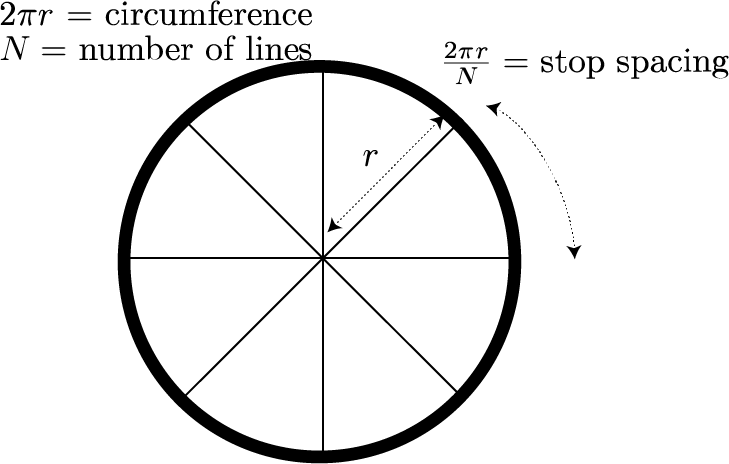
\includegraphics{./walking-time-model.png}
\caption{}
\end{figure}

As before, riders wait on average \(1/2F\) at a stop. If riders start
their journeys evenly distributed around the circle and walk to the
nearest stop, then the average walk distance is \(S/4\) (Convince
yourself!). Therefore, total social cost is

\[
TSC = c_M M + Q\cdot \left[\frac{c_w}{2F} + \frac{c_KS}{4}\right],
\] where the term in brackets is the individual user's wait and walk
time, weighted by \(c_W\) and \(c_K\). Our task is to choose \(N\) and
\(F\) to minimize \(TSC\). To do so, we'll start by eliminating the
variables \(M\) and \(S\).

\subsubsection{\texorpdfstring{Writing \(S\) in terms of
\(N\)}{Writing S in terms of N}}\label{writing-s-in-terms-of-n}

Since bus lines are evenly spaced, and the circumference of the city is
\(2\pi r/N\), then the distance between bus lines is \(2\pi r / N\).
Therefore,

\[S/4=\pi r/2N\]

is the average walk distance.

\subsubsection{\texorpdfstring{Writing \(M\) in terms of \(F\) and
\(N\)}{Writing M in terms of F and N}}\label{writing-m-in-terms-of-f-and-n}

Imagine that you were to stand on an infinitesimal slice of bus-route in
this city---a slice of length \(dx\) miles---and you were to record all
the bus-miles traveled in that slice over one hour. How many bus miles
would you count? Since frequency is \(F\) buses per hour, you would
record \(dx\) bus-miles exactly \(F\) times. And to get the \emph{total}
bus-miles per hour, \(M\), you add the bus-miles measured over all such
slices. There are \(Nr\) miles of bus-routes (look at the picture
above), so that sum can be found by the integral

\[
M = \int_0^{Nr} Fdx,
\]

which is just

\[
M = FNr.
\]

So we have

\[
TSC = c_M FNr + Q\cdot \left[\frac{c_w}{2F} + \frac{c_K\pi r}{2N}\right].
\]

\subsubsection{\texorpdfstring{Solving for \(F^*\) and
\(N^*\)}{Solving for F\^{}* and N\^{}*}}\label{solving-for-f-and-n}

Now we take the first order condition for \(F\) and \(N\).

\[
\frac{\partial TSC}{\partial F}= -\frac{Qc_w}{2F^2} + c_MNr = 0
\]

\[
\frac{\partial TSC}{\partial N}= -\frac{Qc_K\pi r}{2N^2} + c_MFr = 0
\]

Solving these leads to the expressions for optimal \(F\) and
\(N\)\ldots{}

\[
F^* = \sqrt{\frac{c_WQ}{2c_MNr}}
\] and \[
N^* = \sqrt{\frac{c_KQ}{2c_MF}}.
\]

But this isn't the end of the line, because each expression has the
other variable in it. Let's plug the variables into each other's
equations and reduce\ldots{}

\[
F^* = \sqrt{\frac{c_WQ}{2c_Mr \sqrt{\frac{c_KQ}{2c_MF^*}} }} = \left(\frac{c_W}{r c_K}\right)^{2/3}\left( \frac{Q}{2c_M}\right)^{1/3}
\]

\[
N^* = \sqrt{\frac{c_KQ}{2c_M \sqrt{\frac{c_WQ}{2c_MrN^*}} }} = \left(\frac{c_Kr}{c_W}\right)^{2/3}\left( \frac{Q}{2c_M}\right)^{1/3}
\]

Don't get bogged down in all the details here. The important thing is
the power laws\ldots{}

\[
F^*\sim Q^{1/3}
\]

\[
N^*\sim Q^{1/3}
\].

And since \(FNr=M\) is the equation for bus-mileage, this means that

\[
M \sim Q^{2/3}.
\]

\subsection{Takeaways from the model with walk
time}\label{takeaways-from-the-model-with-walk-time}

Don't focus too much on the coefficients and powers here. The takeaway
is this: service should scale more slowly than ridership (because it
scales to the 2/3 power rather than linearly), so you get more people
per bus. It's just that in this model, \(M\) represents service rather
than \(F\), and it scales faster than in the previous model. The reason
is that increasing \(M\) now does two jobs: it reduces wait times
\emph{and} walk times. \(F\) itself scales more slowly than in the
previous model, though, because, for a given \(M\), increasing frequency
means incerasing route spacing (and thus increasing walk times).

    \section{Model 4: boarding time}\label{model-4-boarding-time}

So far we have only focused on the \emph{benefits} of additional riders.
When more people ride, the agency can afford to run more service, which
makes riding more convenient. But there are also downsides to additional
riders. This model deals with one of hte main downsides:
\textbf{boarding time}. It is based on Janson (1979) (in bCourses).

Boarding time is the time it takes passengers to get on the bus. For
simplicity, we're going to leave route spacing out of this model.
Imagine a single bus line that runs between two points, stopping along
the way. Here are the parameters.

\begin{itemize}
\tightlist
\item
  \(Q\) riders/hr
\item
  \(M\) bus-miles/hr
\item
  \(F\) frequency (bus/hr)
\item
  \(D\) route length (mi)
\item
  \(l\) average trip length (mi)
\item
  \(t_B\) boarding time (hr)
\item
  \(c_M\) agency cost of a bus-mile (\$/bus-mile)
\item
  \(c_W\) cost of users' wait time (\$/hr)
\item
  \(c_IV\) cost of users' in-vehicle time (\$/hr)
\item
  \(v\) bus speed between stops (mi/hr)
\item
  \(p\) pace of the bus, counting stops (\(hr/mi\)). `Pace' is a term
  from engineering that tells how long it takes to travel some unit of
  distance.
\end{itemize}

Total social cost is now

\[
TSC = c_MM + Q\left[\frac{c_W}{2F} + c_{IV} l p \right],
\]

where the product \(l p\) is equal to \emph{how long the average
passenger spends on the bus}.

\subsubsection{\texorpdfstring{Writing \(p\) in terms of
frequency}{Writing p in terms of frequency}}\label{writing-p-in-terms-of-frequency}

Let's calculate \(p\) in terms of other variables. To do that, note that
if there are \(M\) bus-miles traveled per hour, and \(Q\) rides per
hour, then a single bus must pick up \(Q/M\) people. Therefore, for
every mile it travels, the bus spends \(1/v\) hrs traveling and
\(t_bQ/M\) sitting still while people board. It follows that

\[
p = \left(\frac{1}{v} + t_B\frac{Q}{M} \right).
\]

\subsubsection{\texorpdfstring{Finding \(F^*\) (optimal
frequency)}{Finding F\^{}* (optimal frequency)}}\label{finding-f-optimal-frequency}

As above, \(M\) is the frequency \(F\) times the total route-mileage.
Above the total route-mileage was \(Nr\); here it's \(D\). So we have

\[
TSC = c_MDF + Q\left[\frac{c_W}{2F} + c_{IV} l \left(\frac{1}{v} + t_B\frac{Q}{DF} \right) \right].
\]

Pause now to remind yourself what each term means. The first is agency
cost. The second is user cost. Within the brackets, the first term is
wait cost, and the second is riding time cost. Now take the first-order
condition on \(F\)\ldots{}

\[
\frac{\partial TSC}{\partial F} = c_M D + Q\left[ -\frac{c_W}{2F^2} - c_{IV}t_Bl \frac{Q}{DF^2} \right] = c_M D - \frac{Q}{F^2}\left[\frac{c_w}{2} + c_{IV}t_Bl \frac{Q}{D} \right] = 0.
\]

Solving for \(F\) gives

\[
F^* = \sqrt{\frac{Q}{c_M D}\left(\frac{c_w}{2} + \frac{t_B c_{IV}lQ}{D} \right)}.
\]

\subsubsection{Takeway from the model with boarding
time}\label{takeway-from-the-model-with-boarding-time}

Now that we've included boarding time, \(F^*\) scales with \(Q\) much
faster than it did without boarding time. Mathematically, that's because
we have the term \((t_B c_{IV}lQ^2)/(D^2)\) inside the parenthesis. But
this should make sense to you intuitively: when passengers take time to
get on the bus, you want to run buses more frequently. Higher frequency
means that there are fewer people on each bus, so the externality
created when each person gets on the bus is smaller; and also each bus
picks up fewer people.

    \section{Takeaway from all the
models}\label{takeaway-from-all-the-models}

We have just looked at four models of simple bus systems. If you're not
used to these types of economic/engineering models, you might be tempted
to ask, ``Which is the most realistic?'' Or ``The most realistic model
would have line spacing \emph{and} boarding time.'' You might think
``These models are worthless because they don't count {[}insert
real-world fact here{]}.''

What I want you to remember, here and throughout the class and even your
careers, is that \textbf{mathematical models are just stories}. They are
really just more logically rigorous versions of Aesop's fables or Zen
koans or ancient myths common in every culture. This isn't just true
because our models involve people: in physics classes you learn about
``free body diagrams'' and ``frictionless surfaces,'' but no such things
have ever existed nor ever will. In every engineering choice you make,
you have to ignore some real facts. The trick is knowing what's relevant
and how you can capture it in a pretty way that illuminates more than it
obscures. For example, if you're designing an airplane, you can operate
in the world of Newtownian physics: forces acting on the plane only
accelerate it. But if you're desining a rocket ship that goes incredibly
fast, you have to take into account relativistic effects whereby the
mass of the vehicle changes as it acquires energy.

So when you look at a model, you have to ask, ``What lesson is this
story trying to tell?'' I think these models have told a few lessons:

\begin{itemize}
\tightlist
\item
  Transit service doesn't just exhibit \emph{physical} scale economies,
  it also has scale economies that arise from the fact transit service
  is provided in particular times and places. The total cost of transit
  service (counting the agency and the users) generally falls as
  ridership rises. That means anything that raises ridership serves a
  broader social purpose: it helps all the people who are already riding
  transit.
\item
  Don't simply increase frequency linearly with ridership, so as to
  maintain a constant load (number of people per bus). Instead, when
  ridership rises, put more people on each bus to save money; and run
  more routes so that people don't have to walk as far.
\item
  Increase frequency more quickly when boarding times are long. That
  way, there are fewer people on each bus who get slowed down when
  another person gets on, and each bus doesn't have to pick up as many
  people.
\end{itemize}


    % Add a bibliography block to the postdoc
    
    
    
    \end{document}
